\section{Database Subsystem}
In this section, we discuss core database concepts like byzantine paxos, role of timestamps in achieving external consistency, distributed transactions and sharding. Concepts that are most new to a database network built for the  decentralized world like distributed query processing, dynamic clustering, data sovereignty and decentralized fine-grained access control are presented.

\subsection{Blockchain consensus}

One of the key questions to answer in a decentralized environment is that of the {\em validity, credibility or
consensus} on a transaction. For example, when a monetary transaction is made among two or more parties, is there consensus among the
involved parties, or among the network as a whole ?

In Picolo, when defining the database schema, it is possible to specify if a consensus is required among the all
participating nodes on the network or only among the participating entities in the application or any combination of
these. It might also be possible to specify a requirement of validation or permission from entities such as regulatory
bodies if they exist in the context of the application.

Once the blockchain grants consensus to a transaction, the credential is captured as a multi-party signed certificate
which can be presented to Picolo to authorize the transaction on the database. Picolo can work with any and all existing
consensus methods used by the major blockchains today. Also for transactions that are public on a public ledger, it
is possible to insert a cryptographic reference to the transaction which would represent a database read operation on
Picolo, thereby making it possible to share the transaction as a link (on a ledger or otherwise).

\subsection{Database Consensus, replication \& sharding} \label{sec:paxos}
All data on \textsf{Picolo} is replicated for durability and high availability. Storage consumers have the option of choosing a replication factor that suits their needs. They can also choose where to locate their data based on where their users are located to achieve better latency or to comply with regulations like GDPR. This data locality can easily be achieved by instructing the network layer to only allow replicas that belong to a geographic region to join the replica group. Consensus is achieved amongst replicas by a running a variant of paxos that is tolerant to byzantine faults.
 \subsubsection{Paxos based replication}
 We modify the algorithms in \cite{byzantine_paxos} to make the leader election more frequent and add a slashing condition that punishes byzantine behavior. There are two roles that each replica can take: \textsf{proposer} and \textsf{acceptor}. Proposers initiate changes to the state by proposing new commands to be appended to a \textsf{sequence} from which the replica state is generated and acceptors vote on which sequence to accept. The system moves through different \textsf{views}. A view can be thought of as a discrete time period (in the order of minutes) with a monotonically increasing view number $\textsf{view}_\textsf{num}$ and has a distinguished proposer called \textsf{leader}. If one imagines that each replica has a number from the set ${1..\mathcal{N}}$ where $\mathcal{N}$ is the number of replicas, then the leader for a view can simply be chosen as $\textsf{leader}_\textsf{view} = \textsf{view}_\textsf{num} \enspace \% \enspace \mathcal{N}$. There are two modes in which the consensus process happens: \textsf{fast} and \textsf{classic}.
\newline\newline
\textbf{Fast mode}: In fast mode (equivalently, \textsf{leaderless mode}), proposers can directly send commands to acceptors bypassing the leader. This obviates the need for \textsf{phase 1b} messages of classic paxos. In a network where replicas are present in distant geographic locations, the savings could be significant. Note that all messages are digitally signed, so the senders can be uniquely identified. A message is a tuple ($\textsf{view}_\textsf{num}$, \textsf{seq}) where \textsf{seq} consists of a prefix - the last accepted command sequence, suffixed with new commands. This differs from the classic paxos algorithm where only scalar values are passed around and offers two major advantages:
\begin{itemize}
	\item Commands need not be exactly similar - commands can appear in differing orders in different replicas as long as they are commutative.
	\item Proposers don't need a promise from acceptors that they will not accept values with a lower \textsf{ballot number} 
\end{itemize}
In the context of a database, two commands are commutative if they are mutating independent records that don't depend on each other for state calculation. For example, reading a row and writing to another row in a table are commutative operations where as reading and writing to the same row may not be. Even writing to different rows if they have different timestamps is non-commutative if \textit{external consistency} is to be maintained (\cref{sec:hybrid_time}). The relaxed definition of command similarity helps replicas achieve consensus quicker compared to the usual case. Since we cannot assume synchronicity of the network, messages may appear in different order at different replicas. So as long as they are commutative, we can tolerate the order difference and proceed with the consensus process. The acceptors always accept a sequence with the highest length, so they don't need to send back the ballot number promise.
\newline\newline
\textbf{Classic mode}: It is possible that the acceptors are unable to make progress in fast mode $i.e$ append new commands to their sequences when they receive concurrent proposals. Since the network is asynchronous and messages may reach out of order, if they are non-commutative and are of the same length, the acceptors cannot agree on the order by themselves. So they fallback to the leader to arbitrage an order for them. They send their sequences to the leader of the current view $\textsf{leader}_\textsf{view}$ who then executes a classic ballot to achieve consensus.
\newline\newline
\textbf{Byzantine fault detection}: Once acceptors receive new proposals, they first verify if the new sequence contains as a prefix an already accepted sequence by them in the past. If not, they simply reject it. If it does, then they sign their acceptance and multicast it to other acceptors. Other acceptors then perform the same check and if it passes, signal their acceptance by $appending$ their signature and multicast it again. This process continues until $\mathcal{N} - f$ acceptors each receive messages with $\mathcal{N} - f$ signatures at which point, the sequence is considered agreed upon and a message is sent back to the proposer indicating consensus. Here $\mathcal{N} \ge 3f+1$. During this process if an honest acceptor receives a multicast that contains signatures of an acceptor $\mathcal{M_A}$ on two non-commutative sequences (see \figref{fig:byz_faults}), then it will trigger a slashing condition (\cref{sec:slashing}). Since we require at least $\mathcal{N} - f$ acceptors to agree on a proposal, at least one of them is guaranteed to be honest and it will trigger the slashing condition. 
\begin{figure}[h!] \centering
	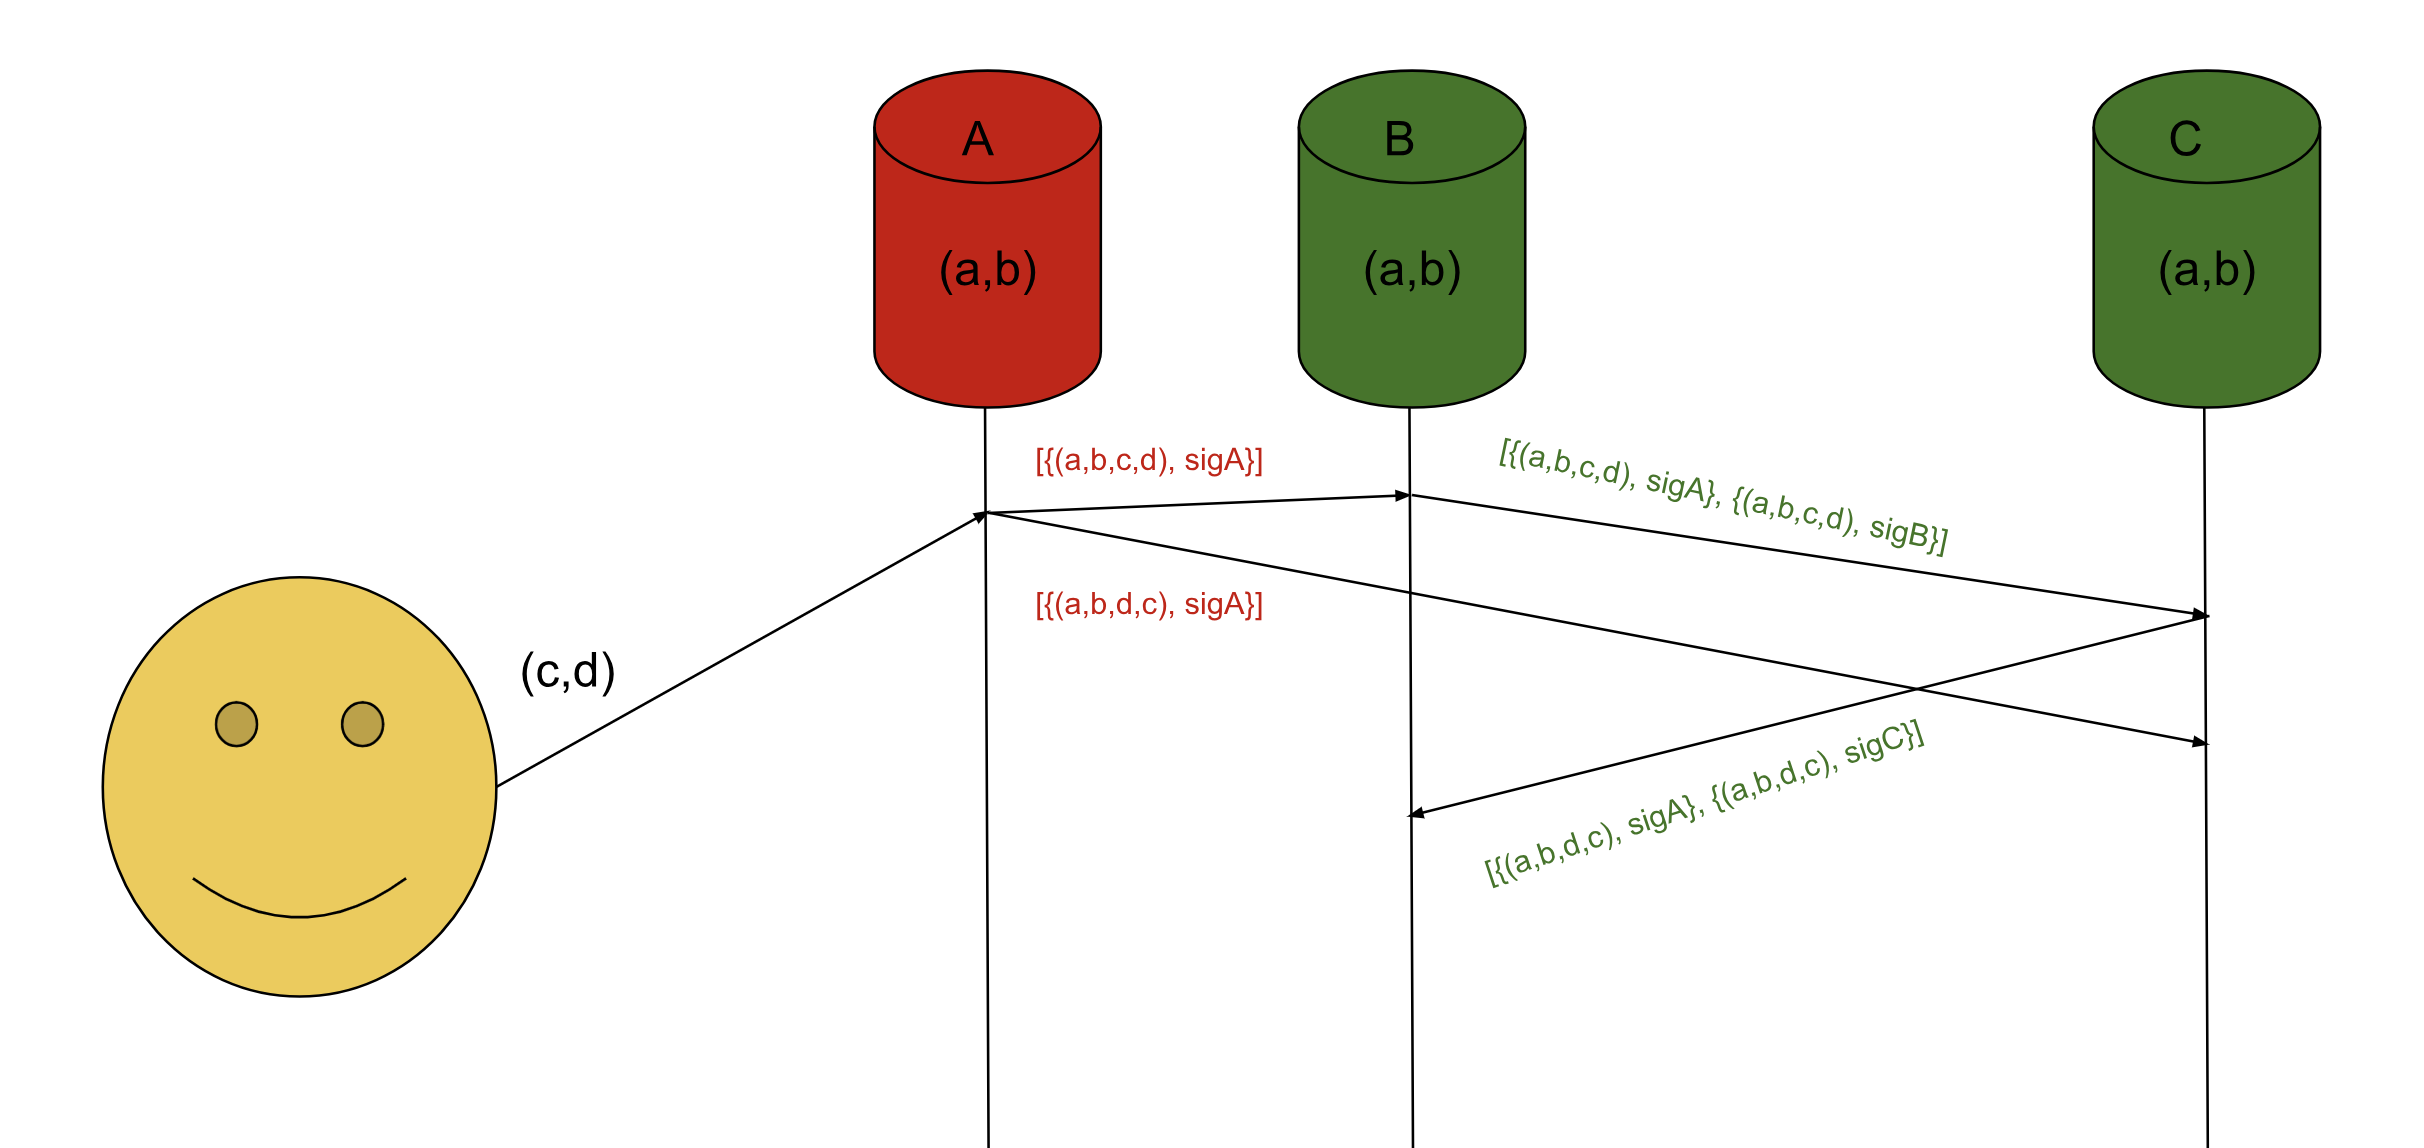
\includegraphics[width=\fscale{0.76}]{byz_faults.png}
	\caption{Byzantine fault detection during Paxos. Replica A sending conflicting messages is detected by B and C}
	\label{fig:byz_faults}
\end{figure}

\subsubsection{Sharding}
\textsf{Picolo} automatically partitions data into multiple shards when it grows too big for any one replica. Each shard consists of a set of key ranges (typically 64MB). A \textsf{key range} is the smallest atomic unit that is replicated aka governed by a paxos group. It is also the smallest unit of movement when data from one replica needs to be sharded into distinct replica sets. The process of sharding is a well studied problem in databases and implementations can be readily found, so we omit a detailed discussion here. 

\subsection{External consistency, Hybrid time \& Distributed transactions} \label{sec:hybrid_time}
Intuitively, external consistency property \cite{External_Consistency} of a distributed system guarantees that the state changes seen by it are exactly in the order applied to it by an external actor. It is the strongest form of consistency a distributed database system can offer and is notoriously hard to achieve in a system with asynchronous network links. Google's Spanner \cite{spanner} achieves this by using the TrueTime api which exposes clock uncertainty as an interval. Every transaction in Spanner has a TrueTime timestamp that indicates its time of entry into the system. Maximum clock uncertainty guaranteed by Truetime is 7ms (due to datacenter latencies); which means by making every transaction wait for 7ms before committing, Spanner can guarantee their total ordering system wide. While these low \textit{commit-wait} latencies (7ms) made possible by state of the art datacenters work fine for Spanner, a decentralized network like \textsf{Picolo} has no such luxuries and needs a new trick.
\subsubsection{Using timestamps}
\textsf{Picolo} uses hybrid time \cite{hybrid_time} - a combination of physical clocks and logical clocks for timestamping. Each node is assumed to provide an accurate enough physical timestamp by running a daemon process that syncs time with NTP stratum 1 servers like Google's external NTP service. If a node's clock is off by more than 500ms from the average of its paxos group, \textsf{Picolo} automatically kills it and finds a replacement. The logical clock is simply a monotonically increasing number appended to the physical time; so its possible to do a simple lexicographic comparison to determine relative order. For each write transaction, $\textsf{leader}_\textsf{view}$ assigns a hybrid timestamp to it before proposing it to replicas. So when two requests r1 followed by r2 hit the same paxos group and pass by $\textsf{leader}_\textsf{view}$, all the replicas are guaranteed to commit requests in the same order irrespective of the order in which they are received. For transactions that span multiple paxos groups, a coordinator (one of the $\textsf{leader}_\textsf{view}$ of individual paxos groups) is elected to perform a \textsf{2 phase commit (2PC)} with other leaders. In the \textsf{prepare} phase of 2PC, each leader acquires locks for its corresponding group and replies with its current timestamp. The coordinator then selects the highest timestamp of all the replies and uses it as the timestamp of the transaction during \textsf{apply} phase. This timestamp is also sent back to the initiator of the transaction so that it can pass it to a subsequent causally related transaction (if any). In the case where this propagation is not possible, external consistency cannot be guaranteed and application developers need to employ the commit wait strategy used by Spanner if desired, although at a performance expense.
\subsubsection{MVCC}
Multi version concurrency control (MVCC) is the practice of storing multiple versions of the same data. In \textsf{Picolo}, each record is uniquely identified by a timestamped key. So keys that differ only by their timestamps represent different versions of the same data. By keeping these different versions, \textsf{Picolo} offers such features as lock-free reads, time travel reads and snapshot isolation. Clients executing read transactions therefore need not acquire any locks since any concurrent writes on the same record have a newer timestamp and won't affect its older timestamped value. Records can also be fetched from the past by specifically executing a read transaction with an older timestamp. For writes however, a lock needs to be acquired on the key being modified. Lock status of keys is stored in a lock table and transactions that mutate data need to check whether the key/range of keys they try to operate on is already present in the lock table, in which case they need to wait. Else, they create an entry in the lock table (thereby acquiring the lock) before proceeding. Similarly, for writes spanning multiple paxos groups, one of the $\textsf{leader}_\textsf{view}$'s is chosen as the coordinator of a \textsf{2PL} (two phase locking) process that facilitates the locking of keys/key ranges of each group by its respective leader.

\subsection{Data in web 3.0}
Our long term goal for \textsf{Picolo} is to make it \textit{the} data network for web 3.0 (\cref{sect:applications}). Data in the new web will be solely controlled by data owners and resides in a single shared network. To support such a network, following capabilities must be built:
\subsubsection{Distributed query processing} \label{sec:dynamic_cluster}
A web 3.0 data network needs to have the capability to execute queries across $all$ nodes in the network in response to a client request. Since nodes will have vastly differing schemas, effective mechanisms for searching and query proessing \cite{query_reformulation, query_processing1, query_processing2} are needed. High level architecture of a \textsf{Picolo} node is depicted in \figref{fig:node_arch}.
\begin{figure}[h!] \centering
	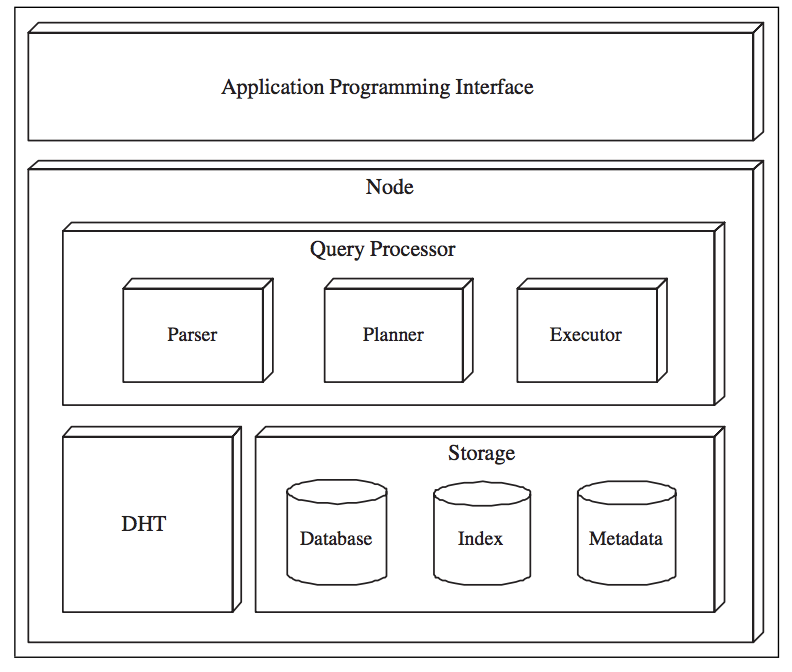
\includegraphics[width=\fscale{0.76}]{node_arch.png}
	\caption{A \textsf{Picolo} node}
	\label{fig:node_arch}
\end{figure}
The schema dictionary depicted in the figure contains metadata to be exposed to the world. Nodes that wish to keep data private should not export the data's metadata to the schema dictionary. Suppose there is a table called \textsf{users} with four columns: \textsf{username}, \textsf{firstname}, \textsf{lastname} and \textsf{email}. The exported metadata entry might look like:
\begin{center}
	\begin{tabular}{| c | c |} 
		\hline
		Entity & Keywords \\ [0.5ex] 
		\hline
		\textsf{users} & user, people, customer, profile\\ 
		\hline
		\textsf{name} & name \\
		\hline
		\textsf{firstname} & fn, {f\_name}, {first\_name} \\
		\hline
		\textsf{lastname} & ln, {l\_name}, {last\_name} \\
		\hline
		\textsf{email} & id, contact \\ [1ex] 
		\hline
	\end{tabular}
\end{center}
When a query is posed to any node in the system, the node first tries to fulfill it with a local query before passing it along to its neighbors. Remember, nodes in the system host data with heterogeneous schemas. Hence the keywords are used to find semantically similar data by assisting in query reformulations.
\newline\newline
\textbf{Dynamic clustering}:
Semantic proximity metrics \cite{PeerDB} and clustering techniques \cite{dynamic_clustering} can be used to find nodes hosting semantically similar schemas. Overtime, these nodes are discovered and are clustered together for better query performance by reducing the number of network hops required.

\subsubsection{Data sovereignty} \label{sec:access_control}
\textsf{Picolo} supports two different schema types: \textit{application controlled} and \textit{user controlled}. Applications can use user controlled schemas to put users in absolute control of data and better comply with regulations like GDPR. For example, a decentralized twitter may  want users to have control over their tweets. Users can use any third party client or \textsf{Picolo}'s official clients to interact with their tweets, effectively rendering the decentralized twitter just another client to the data albeit with better features. \newline\newline
When semantics don't allow to put user in control of data, application controlled schemas can be used. An example here would be a decentralized ticketing application where users should not be given fine grained control to selectively delete data about which tickets they bought.
\newline\newline
\textbf{Access control}:
Applications and users may want to share data with other parties but may wish to impose access controls. There are a few ways of achieving this including building an API on top of the data or using proxy re-encryption techniques. In \cite{ac_p2p_db}, a secret sharing scheme is used instead, where a party given access to encrypted data collects key shares from key holders, reconstructs the key and decrypts data for further use. Acces rules can be defined by a SQL like declarative language at any granularity desired like at the level of a single row or a cell. An example row level granularity rule looks like:\newline \newline
\texttt{SELECT  * \newline FROM users \newline WHERE email=foo@bar.com \newline NODE (SELECT nodeId FROM nodes WHERE domain=application)} \newline \newline
An example value level (only username is given access to) granularity rule looks like:\newline \newline
\texttt{ SELECT username \newline FROM users \newline WHERE email=foo@bar.com \newline NODE (SELECT nodeId FROM nodes)}\newline\newline
Here \texttt{NODE} is a new SQL clause that identifies nodes/actors in the network that have access to the data covered by the rule. Each access rule creates an ecrypted block of data. When there are overlapping rules, multiple encrypted blocks are created with associated keys. The scheme also supports updates to rules - however updates cause data re-encryption and key re-distribution. 

\subsubsection{Role of encryption}
Attribute based encryption (\textsf{ABE}) \cite{abe} was first described by Goyal et.al as a way to achieve fine grained access control on data stored with a third party. It allows attaching policies or access structures to cipher texts and allows decrypting them only if the decryption key has attributes that satisfy the access structure. As an example, in a patient-disease database, a policy could be to allow to only decrypt records where the disease is flu and only keys with the attribute \textit{flu} would be able to decrypt them. \textsf{ABE} comes in two forms: ciphertext-policy ABE (\textsf{CP-ABE}) and key-policy ABE (\textsf{KP-ABE}). In \textsf{CP-ABE}, policies are attached to ciphertexts and attributes are attached to keys whereas in \textsf{KP-ABE}, policies are attached to keys and ciphertexts are labelled with attributes. While these techniques sound promising, there don't seem to be many practical implementations of them in databases. Sieve \cite{sieve} uses \textsf{KP-ABE} to protect user data stored in files with a cloud storage provider. It uses an hybrid encryption scheme where data itself is ecnrypted using a symmetric key and metadata related to the file including its location and the symmetric key is encrypted with \textsf{KP-ABE}. A client first gets the metadata, decrypts it using a key which has a corresponding policy, downloads the file and decrypts it locally with the symmetric key. A similar technique is used in \cite{PPEHR}. The \textsf{ABE} schemes used in either of these systems seem to be secure only under a \textsf{selective-set} model which  may not be sufficient in all adversarial scenarios. Moreover, key revocation in Sieve requires re-encrypting data which may not scale well while in \cite{PPEHR}, the effectiveness of key revocation is not discussed in detail.
\newline\newline
Another body of research focuses on \textsf{ABE} schemes that are \textsf{CCA2} secure. In \cite{cca2_abe1} a \textsf{CCA2} secure \textsf{KP-ABE} scheme is proposed which is based on a \textsf{large universe} construction of another \textsf{KP-ABE} scheme. They overcome the limitations of the underlying scheme by adding a dummy on-the-fly attribute to the decryption procedure which is obtained by running a temporary message through a \textsf{chameleon hash} function. In \cite{cca2_abe2}, authors describe a scheme that is adaptively secure under the complexity assumptions of 3-prime subgroup decision problem. Their scheme allows dynamic update of policies tending itself suitable for practical use cases. But similar to Sieve, the data needs to be re-encrypted by the storage provider (albeit without sacrificing confidentiality). EASiER \cite{easier} is a system that allows for dynamic policy update without the need for data re-encryption. It uses a minimally trusted proxy that faciliates efficient access revocation and can be used in constructing practical systems that use \textsf{ABE} for access control.
\newline\newline
\textsf{Picolo} is the first system that uses \textsf{ABE} for fine-grained access control in a distributed database. It allows data owners to set access rules via the declarative language above and uses a \textsf{CCA2} secure \textsf{ABE} scheme with proxy assisted revocation. \textsf{Picolo}'s construction will be more comprehensively detailed in an upcoming paper.

